\documentclass[12pt]{article}
\usepackage{graphicx}
\usepackage{float}
\usepackage{grffile}
\usepackage{color}
\usepackage{soul}
\usepackage{tabularx}
\usepackage{multirow}
\usepackage{amssymb}
\newcommand{\y}{\checkmark}
% use \xspace to allow for space after a macro as necessary
\usepackage{xspace}
\usepackage[top=1in, bottom=1in, left=1.25in, right=1.25in]{geometry}
\usepackage{pdfpages}
\usepackage{lineno}
%% maxwidth is the original width if it is less than linewidth
%% otherwise use linewidth (to make sure the graphics do not exceed the margin)
\makeatletter
\def\maxwidth{ %
  \ifdim\Gin@nat@width>\linewidth
    \linewidth
  \else
    \Gin@nat@width
  \fi
}
\makeatother

\definecolor{commentcol}{rgb}{0.345, 0.345, 0.945}
\newcommand{\comment}[1]{\textcolor{commentcol}{[[#1]]}}%

% general-purpose mathrm macros
\newcommand{\symsub}[2]{\ensuremath{#1_{\tiny \mathrm{#2}}}\xspace}
\newcommand{\mrm}[1]{\ensuremath{\mathrm{#1}}
\xspace}

\usepackage{framed}
\makeatletter
\newenvironment{kframe}{%
 \def\at@end@of@kframe{}%
 \ifinner\ifhmode%
  \def\at@end@of@kframe{\end{minipage}}%
  \begin{minipage}{\columnwidth}%
 \fi\fi%
 \def\FrameCommand##1{\hskip\@totalleftmargin \hskip-\fboxsep
 \colorbox{shadecolor}{##1}\hskip-\fboxsep
     % There is no \\@totalrightmargin, so:
     \hskip-\linewidth \hskip-\@totalleftmargin \hskip\columnwidth}%
 \MakeFramed {\advance\hsize-\width
   \@totalleftmargin\z@ \linewidth\hsize
   \@setminipage}}%
 {\par\unskip\endMakeFramed%
 \at@end@of@kframe}
\makeatother

\definecolor{randomcolor}{rgb}{.97, .27, .67}
\definecolor{shadecolor}{rgb}{.97, .97, .97}
\definecolor{messagecolor}{rgb}{0, 0, 0}
\definecolor{warningcolor}{rgb}{1, 0, 1}
\definecolor{errorcolor}{rgb}{1, 0, 0}
\newenvironment{knitrout}{}{} % an empty environment to be redefined in TeX

\usepackage{alltt}
%% hard to sort by year automatically ...
%% https://tex.stackexchange.com/questions/377449/sorting-citations-and-bibliography-using-natbib-and-plainnat?rq=1
\usepackage[sort]{natbib}
\usepackage{blkarray}
\usepackage{bm}
\usepackage{amsmath,empheq}
\usepackage{alltt}
\usepackage{hyperref}
\usepackage[utf8]{inputenc} % for accented characters
%% stuff for editing
%\usepackage[markup=nocolor,addedmarkup=bf,deletedmarkup=sout]{changes}
%% to suppress notes & comments: \usepackage[final]{changes}
\usepackage{setspace}
\usepackage{changes}
\usepackage[backgroundcolor=lightgray,textsize=tiny]{todonotes}

\bibliographystyle{chicago}
\title{Reformulating phylogenetic mixed models to improve flexibility and speed}
\author{Michael Li and Ben Bolker}
\date{\today}

\providecommand{\keywords}[1]{\textbf{\textit{Keywords:}} #1}
\IfFileExists{upquote.sty}{\usepackage{upquote}}{}
 \vspace{-8ex}
  \date{}
\begin{document}
\newcommand{\dbic}{\ensuremath \Delta \textrm{BIC}}

%% don't typeset BMB comments
\newcommand{\bmbhide}[1]{}
\newcommand{\bmb}[1]{{\color{blue} BB: #1}}


\renewcommand{\figurename}{Fig.}

\newcommand{\mli}[1]{{\color{red} ML: #1}}

\newcommand{\add}[1]{{\color{blue} ADD: #1}}


\newcommand{\pkg}[1]{{\tt #1}}
\newcommand{\code}[1]{{\tt #1}}


% \pagenumbering{gobble}
\linenumbers

% \renewcommand{\bmb}[1]{\relax}
% \renewcommand{\mli}[1]{\relax}



%\SweaveOpts{concordance=TRUE}
%\SweaveOpts{concordance=TRUE}
% \maketitle

\begin{center}
{\Large
\textbf\newline{Reformulating phylogenetic mixed models to improve flexibility and speed} % Please use "sentence case" for title and headings (capitalize only the first word in a title (or heading), the first word in a subtitle (or subheading), and any proper nouns).
}
% Insert author names, affiliations and corresponding author email (do not include titles, positions, or degrees).
\\
\vspace{2pt}
Michael Li\textsuperscript{1*} and Benjamin M. Bolker\textsuperscript{1,2,3}
\\
\vspace{2pt}
* Corresponding author: Michael Li; lim88@mcmaster.ca
\end{center}
\vspace{5pt}
\textbf{1} Department of Biology, McMaster University, Hamilton, Ontario, Canada
\\
\textbf{2} Department of Mathematics and Statistics, McMaster University, Hamilton, Ontario, Canada
\\
\textbf{3} Institute for Infectious Diseases Research, McMaster University, Hamilton, Ontario, Canada
\\
\bigskip

\doublespacing


\section*{Abstract}

\begin{enumerate}
\item{Phylogenetic regression is a powerful technique for exploring relationships among characteristics of related species. However, existing procedures may be either insufficiently flexible or too computationally demanding when analyzing large volumes of data.}
\item{We propose an alternative formulation of phylogenetic generalized linear mixed models that is mathematically equivalent to previous approaches, but is more flexible in practice. We have implemented this formulation in two R statistical packages (\pkg{lme4} and \pkg{glmmTMB}).}
\item{Our reformulation of phylogenetic generalized linear mixed models is computationally efficient, operating orders of magnitude faster than existing comparably flexible methods.}
\item{Our approach can be implemented in any platform for generalized mixed models. Our implementation in \pkg{lme4} and \pkg{glmmTMB} allows users to fit phylogenetic mixed models to a broad range of previously difficult cases (e.g., large data, unbalanced observational designs, complex random effects).}
\end{enumerate}

\keywords{phylogenetic comparative methods, phylogenetic correlation, phyloglmm, species--branch matrix}




\section*{Introduction}

Phylogenetic comparative methods (PCMs) account for evolutionary relatedness when analyzing species traits.
Given a known phylogeny, PCMs model the relationships among species traits while incorporating relatedness; they can be used to control statistically for phylogeny, to quantify phylogenetic signal in traits, or both. 

In contrast to standard statistical models, where all of the predictor variables (such as species traits and environmental covariates) are directly observable, PCMs use phylogenetic relationships to incorporate the unobserved process of trait evolution \citep{felsenstein1985phylogenies, butler2004phylogenetic, hansen2012interpreting}. 
While a wide range of tools is available for PCM, existing procedures are either insufficiently flexible or too computationally demanding to analyze large data sets.
When faced with these constraints, researchers often simplify their analyses, at the risk of neglecting important processes.

\subsection*{Challenges in modeling phylogenetic processes}

In classic PCMs, phylogenetic correlation in the residuals from a regression between two species-level traits arises because the residual variation in the response trait evolves along the branches of the phylogeny according to a Brownian-motion (BM) evolutionary model \citep{felsenstein1985phylogenies}. 
If the residuals are normally distributed and observed without additional error or within-species variation, Felsenstein's method of phylogenetically independent contrasts  \citep[PICS:][]{felsenstein1985phylogenies} is sufficient to account for the phylogenetic correlation.
More recent approaches --- including phylogenetic generalized linear mixed models (PGLMM) \citep{ives2011generalized, housworth2004phylogenetic}, Pagel's $\lambda$ \citep{pagel1999inferring}, and Blomberg's $K$ \citep{blomberg2003testing} --- extend PICs by considering different (non-Gaussian) response distributions and by accounting for evolutionary models other than BM.
These methods partition residual variation into two components: (1) independent residual variation (tip variation, which is confounded with observation error) and (2) phylogenetic signal (evolutionary process error) \citep{hansen2012interpreting, housworth2004phylogenetic}.
If each species' traits are measured multiple times, we can distinguish a third level of variation; in this case, phylogenetic variation and tip variation are both part of the evolutionary process error while the observation error can be independently identified from within-species variation.
Although many studies include multiple observations per species, phylogenetic analyses rarely take advantage of such information to partition variability more finely.

Classic PCMs allow the residuals to evolve along the phylogeny, but the effects of the predictor variables may evolve along the phylogeny as well; extending PCMs to allow for multiple sources of variation leads to the  \emph{phylogenetic mixed model} \citep{housworth2004phylogenetic}.
For example, suppose we wish to fit a PCM to predict species' brain size from their body size \cite{felsenstein1985phylogenies} using a mixed-effect model.
The standard PCM allows for phylogenetic correlations in the residuals of the relationship between body and brain size; the phylogenetic mixed model can allow incorporate both
variation in brain size among taxa with similar body sizes (random intercepts) and
variation in the \emph{relationship} between predictors and responses among taxa (random slopes).

Several recent studies have used phylogenetic mixed models in
community ecology \citep{nowakowski2018phylogenetic, li2017canfun}.
However, the phylogenetic mixed modeling tools that allow extensions such as random slopes
and separation of tip and observation error in a frequentist framework are inflexible; thus, biologists needing to fit random-slopes models typically turn to Bayesian approaches, despite their additional computational burden \citep{hadfield2010mcmc, burkner2018brms} (Table \ref{table:model}).

\begin{table}[]
\begin{tabular}{|l|l|l|l|}
\hline
\textbf{Model} & \textbf{Method} & \textbf{Data} & \textbf{Platform} \\ \hline
\multirow{2}{*}{
\begin{tabular}[c]{@{}l@{}}Generalized Linear \\ Model (GLM)
\end{tabular}} & Correlated residual & \begin{tabular}[c]{@{}l@{}}Single observation \\ per species \end{tabular} & \begin{tabular}[c]{@{}l@{}}\pkg{nlme}:gls, \\ \pkg{ape}:pic\end{tabular} \\ \cline{2-4} 
& \begin{tabular}[c]{@{}l@{}}Residual \\ + phylogenetic intercept\end{tabular} & \begin{tabular}[c]{@{}l@{}}Single observation \\ per species \end{tabular} & \begin{tabular}[c]{@{}l@{}}Pagel's $\lambda$\\ Blomberg's $k$ \\ via \pkg{nlme}:gls\\ \pkg{phylolm}\end{tabular} \\ \hline
\multirow{2}{*}{\begin{tabular}[c]{@{}l@{}}Generalized Linear \\ Mixed Model (GLMM)\end{tabular}} & \multirow{2}{*}{Random effect}                                        & \begin{tabular}[c]{@{}l@{}}Single observation \\per species, \\ Balanced design\end{tabular} & \pkg{pez}                                                                                            \\ \cline{3-4} 
                                                                                                  &                                                                       & Unrestricted                                                                 & \pkg{lme4}, \pkg{glmmTMB}, \pkg{phyr}                                                                                  \\ \hline
\multirow{2}{*}{Bayesian GLMM}                                                                    & \multirow{2}{*}{Random effect}                                        & Balanced design                                                              & \pkg{MCMCglmm}                                                                                       \\ \cline{3-4} 
                                                                                                  &                                                                       & Unrestricted                                                                 & \pkg{brms}                                                                                           \\ \hline
\end{tabular}
\caption{GLM-based phylogenetic comparative methods and their implementations in R packages.}
\label{table:model}
\end{table}

We propose an alternative, more flexible formulation of the phylogenetic mixed model that is mathematically equivalent to previous approaches.
In particular, it allows for complex phylogenetic effects (random intercepts, slopes, and interactions), without the need to implement special correlation structures, by incorporating phylogenetic structures as part of the mean model \citep{hefley2017basis}.
We compare our technique (built on the R packages \pkg{lme4} and \pkg{glmmTMB}) with existing R packages, fitting models to simulated data that incorporates random slopes, random intercepts (tip variation), and residual variation.

\section*{Materials and Methods}

\newcommand{\bX}{{\mathbf X}}
\newcommand{\bbeta}{{\boldsymbol \beta}}
\newcommand{\bmu}{{\boldsymbol \mu}}
\newcommand{\bY}{{\mathbf y}}  %% fixme later
\newcommand{\bC}{{\mathbf C}}
\newcommand{\bZ}{{\mathbf Z}}
\newcommand{\bb}{{\mathbf b}}
\newcommand{\besp}{{\boldsymbol \epsilon}}
\newcommand{\bSigma}{{\boldsymbol \Sigma}}

\subsection*{Phylogenetic regression}

Suppose a species trait $\bY$ is a linear function of some predictors encoded in a model matrix $\bX$, where each species is measured exactly once. 
The standard phylogenetic regression can be expressed as
\begin{equation}
\begin{aligned}
\bY & = \bX \bbeta + \besp  \\
\besp & \sim \textrm{MVN}(0,\sigma^{2} \bC), 
\label{eq:gls}
\end{aligned}
\end{equation}
where $\bY$ is an length-$n$ response vector; $\bX$ is an $n \times m$ matrix, describing $n$ observations of $m$ predictor variables; $\bbeta$ is an $m$-vector of coefficients; $\besp$ is a multivariate normally distributed $n$-vector with mean $0$ and covariance matrix $\sigma^{2} \bC$ where $\bC$ is a $n \times n$ phylogenetic correlation (PC) matrix that quantifies the proportion of shared evolution between any pair of taxa in the phylogeny \citep{garamszegi2014modern}.

\subsection*{Phylogenetic generalized linear mixed model}

The phylogenetic generalized linear mixed model (PGLMM) framework defines a wider range of models that includes the standard phylogenetic regression as a special case \citep{lynch1991methods}.
The PGLMM allows for non-Gaussian responses and uses incorporates multiple components of variability.
The PGLMM has the form:
\newcommand{\dist}{{\cal D}}
\begin{equation}
\begin{aligned}
\bY & = \dist(g^{-1}(\bmu), \phi) \\
\bmu & = \bX \bbeta + \bZ \bb  \\
\bb & \sim \textrm{MVN}(0, \bSigma(\theta))  \\
\label{eq:glmm}
\end{aligned}
\end{equation}
where in addition to the terms from (\ref{eq:gls}) $\bZ$ is an $n \times q$ model matrix for the $q$-dimensional vector-valued random effects; $\bb$ represents the conditional mean (or mode) of the random effect, which is multivariate normally distributed with covariance matrix $\bSigma(\theta)$; and $\phi$ is a scale parameter for the conditional distribution $\dist$.
When $\dist$ is Gaussian, $g$ is the identity function, $\bZ$ is the identity matrix, and $\bSigma(\theta)=\sigma^2\bC$, (\ref{eq:glmm}) reduces to (\ref{eq:gls}).

\subsection*{Reformulating the phylogenetic covariance matrix}

\newcommand{\bS}{{\mathbf S}}
\newcommand{\bJ}{{\mathbf J}}
\newcommand{\bB}{{\mathbf B}}
\newcommand{\bBadj}{{\mathbf B}_{\mbox{\tiny adj}}}
\newcommand{\bomega}{{\boldsymbol \omega}}
\newcommand{\bell}{{\boldsymbol \ell}}
\newcommand{\e}{{ \epsilon}}

In general, correlations within statistical models can be integrated either in the 
covariance matrix $\bSigma$ or in the structure of the model matrix $\bZ$ \citep{hefley2017basis};
thus, we can use $\bZ$ to incorporate phylogenetic correlations.
Suppose evolution follows a BM process, i.e., continuous traits evolve independently, following an unbiased random walk along each branch of the phylogeny.
Then the phylogenetic variability of a particular species can be written as the sum of the variances of evolutionary changes that occurred on all of the branches in its history. 
Thus, modeling the evolutionary history of each species with a sequence of independent errors with species--branch matrix $\bS$ is equivalent to imposing a correlation $\bC$.
For example, for the phylogeny in figure \ref{fig:tree}, the corresponding $\bS$ takes the form:

\begin{center}
\begin{figure}[H]
  \includegraphics[scale=0.8,page=1]{./figure/phylotree.png}
  \caption{Three-species phylogenetic tree.}
\label{fig:tree}
\end{figure}
\end{center}
\[
  \begin{blockarray}{ccccc}
  & L_1 & L_2 & L_3 & L_4  \\
  \begin{block}{c(cccc)}
  t_1 & \ell_1 & \ell_2 & 0           & 0 \\
  t_2 & \ell_1 &  0          & \ell_3 & 0 \\
  t_3 & 0           &  0          & 0           & \ell_4 \\
  \end{block}
  \end{blockarray}
  \hspace{0.5cm}
  \begin{blockarray}{c}
    \vphantom{L_1} \\
    \begin{block}{(c)}
      \e_1 \\
      \e_2 \\
      \e_3 \\
      \e_4 \\
    \end{block}
  \end{blockarray}
  \]
% \begin{pmatrix}
% \e_1 \\
% \e_2 \\
% \e_3 \\
% \e_4
% \end{pmatrix}
%% FIXME: double check this
For example, the phylogenetic effect for species 1 is $\ell_1 \e_1 + \ell_2 \e_2$, where $\ell_i = \sqrt{L_i}$, the square root of the branch length $L_i$ in Figure \ref{fig:tree}, and the $\e_i$ are independent Normal deviates with zero mean and variance $\sigma^2$ (i.e. the phylogenetic variance for species 1 is $\textrm{E}[(\ell_1 \e_1 + \ell_2 \e_2)^2] = (L_1 + L_2)\sigma^2$).
% The variance of Brownian-motion, is the evolutionary rate, where it is linear in evolution time.

\subsubsection*{Constructing the species--branch random effects model matrix}

The $\bS$ matrix is the product of an $m \times b$ indicator matrix $\bS_{ind}$ of branch indices and a vector $\bell$ of square roots of branch lengths:

\[
\bS_{ind} = \begin{bmatrix}
1 & 1 & 0 & 0 \\ 
1 & 0 & 1 & 0 \\ 
0 & 0 & 0 & 1
\end{bmatrix} , 
\qquad
\bell = \begin{bmatrix}
\ell_1 \\
\ell_2 \\
\ell_3 \\
\ell_4 
\end{bmatrix} .
\]
$\bS_{ind}$ is a binary (indicator) matrix that describes whether a particular branch occurs in the history of a focal species. 
$\bS \bS^T$ gives the covariance matrix of the phylogeny. 

In general, the random-effect model matrix $\bZ$ for a mixed model can be decomposed into term-wise model matrices $\bZ_{i}$ as described in \citet{bates2015fitting}.
Analogous to this procedure, the phylogenetic random-effect matrix $\bZ^{C}_{i}$ is

\begin{equation}
\bZ^{C}_{i} = (\bS^{\top}\bJ^{\top}_{i} \ast \bX^{\top}_{i})^{\top}, \label{eq:ZC}
\end{equation}
where $\bS$ is the $m \times b$ species--branch matrix; $\bJ_{i}$ is the $n_i \times m$ indicator matrix of grouping factors; $\bX_{i}$ is the $n \times p_{i}$ raw random-effects model matrix; and $\ast$ is the Khatri-Rao product \citep{khatri1968solutions} partitioned at the observation level ($n$).

For example, using the phylogeny above (figure \ref{fig:tree}), if we begin with a model matrix corresponding to intercept and slope terms, 

\[
\bX = \begin{bmatrix}
1 & t_1  \\ 
1 & t_2  \\ 
1 & t_3 
\end{bmatrix} 
\]
then the term-wise phylogenetic random effects model matrix is,

\begin{equation}
\begin{aligned}
\bZ^{C}_{i} = (\bS^{\top}\bJ^{\top}_{i} \ast \bX^{\top}_{i})^{\top} =
\left[
\left(
\begin{bmatrix}
\ell_{1} & \ell_{1}  & 0 \\
\ell_{2} &  0  & 0 \\
0  &  \ell_{3} & 0 \\
0 & 0 &  \ell_{4} 
\end{bmatrix}
\begin{bmatrix}
1 & 0  & 0 \\
0 & 1  & 0 \\
0 & 0  & 1  
\end{bmatrix}
\right)
\ast
\begin{bmatrix}
1   & 1   & 1  \\ 
t_1 & t_2 & t_3
\end{bmatrix} 
\right]^{\top}
\\
= \begin{bmatrix}
\ell_{1} & \ell_{1}t_1 & \ell_{2} & \ell_{2}t_1 & 0 & 0 & 0 & 0 \\
\ell_{1} & \ell_{1}t_2 & 0 & 0 & \ell_{3} & \ell_{3}t_2 & 0 & 0 \\
0 & 0 & 0 & 0 & 0 & 0 & \ell_{4} & \ell_{4}t_3
\end{bmatrix}.
\end{aligned}
\end{equation}

\subsection*{Simulation}
\subsubsection*{Single group model}

We generated test data based on (\ref{eq:glmm}) with a single response variable $\bY$ and a single normally distributed predictor variable $\bm{t}$ for $n$ = 25, 50, and 100 species.
The response variable $\bY$ is conditionally normally distributed (i.e., $\cal{D}$ is a Gaussian distribution, and $g$ is the identity link function), corresponding to a linear mixed effect model. 
For the first set of simulations, we simulate one observation per species.
% For a broader range of comparisons, we simulate one observation ($X_i,Y_i$) per species.
Thus, the full simulation model is as follows:
\begin{equation}
\begin{aligned}
\bY & = \dist(g^{-1}(\bmu), \phi) \\
\bmu & = (\bf{\beta_0 + b_{\mathrm{phy_{int}}}}) + (\bf{\beta_1 + b_{\mathrm{phy_{slope}}}}) \bm{t} + \besp \\\
(\bf{b_{\mathrm{phy_{int}}}, b_{\mathrm{phy_{slope}}}}) & \sim \textrm{MVN} \left( 0, \begin{bmatrix}
\Sigma^2_{\mathrm{phy_{int}}} & \Sigma_{\mathrm{phy_{int-slope}}} \\ 
\Sigma_{\mathrm{phy_{int-slope}}} & \Sigma^2_{\mathrm{phy_{slope}}}
\end{bmatrix} 
\right) \\ 
\besp & \sim \textrm{N} ( 0 , \sigma_{\epsilon}^2) \quad.
\label{eq:single_glmm}
\end{aligned}
\end{equation}
The model has two fixed effect parameters ($\beta_0$ and $\beta_1$), three random effect parameters (phylogenetic random intercept variance $\Sigma^2_{\mathrm{phy}_{int}}$, phylogenetic random slope variance $\Sigma^2_{\mathrm{phy}_{slope}}$ and covariance between phylogenetic random intercept and slope $\Sigma_{\mathrm{phy_{int-slope}}}$) and residual variance ($\sigma_{\epsilon}^2$).  
The covariance between phylogenetic random intercept and slope measures the correlation of phylogenetic effects on the slope ($b_{\mathrm{phy_{slope}}}$) and intercept ($b_{\mathrm{phy_{int}}}$) for each branch of the phylogeny; i.e. a positive correlation indicates that species with similar intercepts also have similar slopes.
Predictor-level and intercept-level random effects of species are not applicable in this simulation setting because there is only a single observation per species, so within-species variation cannot be separated from tip variation.

\subsubsection*{Multi-group model}

We extend the simulation model by adding multiple groups where each group has one observation per species. 
The multi-group model is a generalization of multiple-site models used in community ecology to model phylogenetic attraction \citep{helmus2007separating}. 
The full multi-group model is as follows: 
\begin{equation}
\begin{aligned}
\bY & = \dist(g^{-1}(\bmu), \phi) \\
\bmu & = (\bf{\beta_0 + b_{\mathrm{phy_{int}}} + b_{\mathrm{sp_{int}}} + b_{\mathrm{group}}}) + (\bf{\beta_1 + b_{\mathrm{phy_{slope}}} + b_{\mathrm{sp_{slope}}}}) \bm{t} + \bf{b_{\mathrm{sp:group}}} + \besp \\
(\bf{b_{\mathrm{phy_{int}}}, b_{\mathrm{phy_{slope}}}}) & \sim \textrm{MVN} \left( 0, \begin{bmatrix}
\Sigma^2_{\mathrm{phy_{int}}} & \Sigma_{\mathrm{phy_{int-slope}}} \\ 
\Sigma_{\mathrm{phy_{int-slope}}} & \Sigma^2_{\mathrm{phy_{slope}}}
\end{bmatrix}
\right) \\
(\bf{b_{\mathrm{sp_{int}}}, b_{\mathrm{sp_{slope}}}}) & \sim \textrm{MVN} \left( 0, \begin{bmatrix}
\sigma^2_{\mathrm{sp_{int}}} & \sigma_{\mathrm{sp_{int-slope}}} \\ 
\sigma_{\mathrm{sp_{int-slope}}} & \sigma^2_{\mathrm{sp_{slope}}}
\end{bmatrix}
\right) \\
\bf{b_{\mathrm{group}}} & \sim \textrm{MVN} ( 0 , \sigma^2_{\mathrm{group}}) \\
\bf{b_{\mathrm{sp:group}}} & \sim \textrm{MVN} (0, \mathrm{I}_{\mathrm{group}} \otimes \Sigma^2_{phy}) \\
\besp & \sim \textrm{N} ( 0 , \sigma_{\epsilon}^2),
\label{eq:multiple_glmm}
\end{aligned}
\end{equation}
where $\textrm{I}_{\textrm{group}}$ is a indicator matrix for groups and $\otimes$ is the Kronecker product.

Compared to the single--group model, the multi-group simulation model has five additional random effect parameters (predictor-level ($\sigma^2_{\mathrm{sp_{slope}}}$) and intercept-level ($\sigma^2_{\mathrm{sp_{int}}}$) random effect of species variance and their covariance ($\sigma_{\mathrm{sp_{int-slope}}}$), random intercept of group ($\bf{b_{\mathrm{group}}}$) and random intercept of species-group interaction ($\bf{b_{\mathrm{sp:group}}}$))
Because each species has multiple observations we can distinguish variation among species from residual variation, and thus we can include predictor-level and intercept-level random effects of species.
Variance in the intercept of species--group interactions ($\bf{b_{\mathrm{sp:group}}}$) describes whether the species within a group have more similar responses on average than expected by chance, equivalent to phylogenetic attraction \citep{helmus2007separating}. 

\subsection*{Platforms}

We compare our approach with five other R packages that can fit PCMs: \pkg{nlme} \citep{pinheiro2014r}, \pkg{phylolm} \citep{ho2014phylolm}, \pkg{pez} \citep{pearse2015pez}, \pkg{phyr} \citep{phyr} and \pkg{brms} \citep{burkner2018brms}.
Phylogenetic generalized least squares (PGLS) (\code{gls} in \pkg{nlme}) is one of the most widely used PCM models; it fits a linear model with a covariance structure that assumes an evolutionary process on the tree (typically BM, but other processes can be used) instead of treating the residual error for each species as independent.
Phylogenetic generalized linear models (PGLM) (\code{phyloglm} in the \pkg{phylolm} package) are extend PGLS by allowing for both phylogenetic and residual variation, as well as non-Gaussian response variables.
Both \code{gls} and \code{phylolm} can model non-Brownian evolutionary processes and different correlation structures (e.g., Pagel's $\lambda$ or Blomberg's $K$), but we restrict our PGLS fits to the simple BM correlation.
Neither PGLS nor PGLM can handle random slopes or multiple observations within a species.
Among the few packages that currently fit phylogenetic slopes to predictor level variation are \pkg{pez} and \pkg{phyr}, which can handle random-slope models ($\Sigma^2_{\mathrm{phy_{slope}}}$) and random intercepts of species-group interactions ($\bf{b_{\mathrm{sp:group}}}$) but do not incorporate covariation between phylogenetic random slopes and intercepts ($\Sigma_{\mathrm{phy_{int-slope}}}$).
Lastly, Bayesian PGLMMs using Markov chain Monte Carlo (MCMC) can handle all of the cases described above. 
However, MCMC is usually much more computationally expensive for GLMMs than platforms using deterministic optimization.
\pkg{MCMCglmm} \citep{hadfield2010general} is the most widely used Bayesian phylogenetic GLMM, but we will instead use \pkg{brms}, which uses a more computationally efficient MCMC technique.
 
% Table \mli{ref something} provides the statistically equivalent fitting capabilities of common/existing phylogenetic methods.
\begin{table}[]
\resizebox{\textwidth}{!}{%
\begin{tabular}{|c|c|c|c|c|c|c|c|}
\hline
 & \pkg{nlme} & \pkg{phylolm} & \pkg{lme4}/\pkg{glmmTMB} & \pkg{pez} & \pkg{phyr} & \pkg{brms} & \pkg{MCMCglmm} \\ \hline
Single Group & \y & \y & \y &  &  & \y & \y \\ \hline
\begin{tabular}[c]{@{}c@{}}Phylo Intercept\\ Phylo Slope\\ Phylo Slope-Intercept correlation\\ Residual\end{tabular} & \y & \begin{tabular}[c]{@{}c@{}}\y\\ \\ \\ \y\end{tabular} & \begin{tabular}[c]{@{}c@{}}\y\\ \y\\ \y\\ \y\end{tabular} &  &  & \begin{tabular}[c]{@{}c@{}}\y\\ \y\\ \y\\ \y\end{tabular} & \begin{tabular}[c]{@{}c@{}}\y\\ \y\\ \y\\ \y\end{tabular} \\ \hline
Multi-group &  &  & \y & \y & \y & \y & \y \\ \hline
\begin{tabular}[c]{@{}c@{}}Phylo Intercept\\ Phylo Slope\\ Phylo Slope-intercept correlation\\ Phylo Species-group interaction\\ Species intercept\\ Species Slope \\ Species Slope-intercept correlation\\ Residual\end{tabular} &  &  & \begin{tabular}[c]{@{}c@{}}\y\\ \y\\ \y\\ \y\\ \y\\ \y\\ \y\\ \y\end{tabular} & \begin{tabular}[c]{@{}c@{}}\y\\ \y\\ \\ \y\\ \y\\ \y\\ \\ \y\end{tabular} & \begin{tabular}[c]{@{}c@{}}\y\\ \y\\ \\ \y\\ \y\\ \y\\ \\ \y\end{tabular} & \begin{tabular}[c]{@{}c@{}}\y\\ \y\\ \y\\ \y\\ \y\\ \y\\ \y\\ \y\end{tabular} & \begin{tabular}[c]{@{}c@{}}\y\\ \y\\ \y\\ \\ \y\\ \y\\ \y\\ \y\end{tabular} \\ \hline
\end{tabular}%
}
\caption{List of estimable parameters for each R package.}
\label{table:platform}
\end{table}

\subsection*{Simulation and evaluations}

Using the R package \pkg{ape} \citep{ape}, we simulated 100 random phylogenetic trees  for each sample size (n = 25, 50, 100 and an additional n = 500 for the multi-group model) and then simulated the responses for each tree (\ref{eq:single_glmm}, \ref{eq:multiple_glmm}). 
Each realization was fitted using all model variants. 
All simulation parameters are shown in Figure \ref{ssplot} and Figure \ref{msplot}. 
We parameterize the models with correlation $\rho_{xy}$ rather than covariance $\Sigma_{xy}$ (i.e., $\rho_{xy} = \frac{\Sigma_{xy}}{\Sigma_{x}\Sigma_{y}}$).
%\bmb{???}
%mli{Just to match what lme4/glmmtmb outputs.}
Table \ref{table:platform} shows the parameters that are estimable for each platform. 
We only evaluated the goodness of fit for model fits that passed the convergence tests implemented by the package.
For Bayesian fits, we evaluate realizations with Gelman-Rubin statistic $<1.1$. Based on recent concerns about Gelman-Rubin thresholds \citep{vats2018revisiting}), we additionally restricted results to fits with  effective sample size $>1000$ for the fixed effect parameters ($\beta_{0}$ and $\beta_{1}$) \citep{vehtari2019rank}. 
For each replicate, we sample two chains starting with 10000 iterations. 
We first evaluate our estimates by looking at the distribution of the estimated values (maximum likelihood estimates for non-Bayesian platforms and posterior medians for Bayesian platforms) to quantify bias and variance (i.e., quality of the point estimate).
We computed 95\% Wald confidence intervals for frequentist methods and quantile-based intervals for Bayesian methods, then computed coverage --- the proportion of simulations in which the computed confidence intervals include the true values of parameters --- to assess the quality of the confidence intervals.
We also compare computational speed between different platforms to evaluate the efficiency of different platforms and methods. 

In supplementary materials, we reproduce the examples in chapter 11 of \cite{garamszegi2014modern} using phylogenetic GLMMs based on \pkg{lme4} and \pkg{glmmTMB}.

\section*{Results}

\subsection*{Single Group model simulations}

\begin{center}
\begin{figure}[H]
  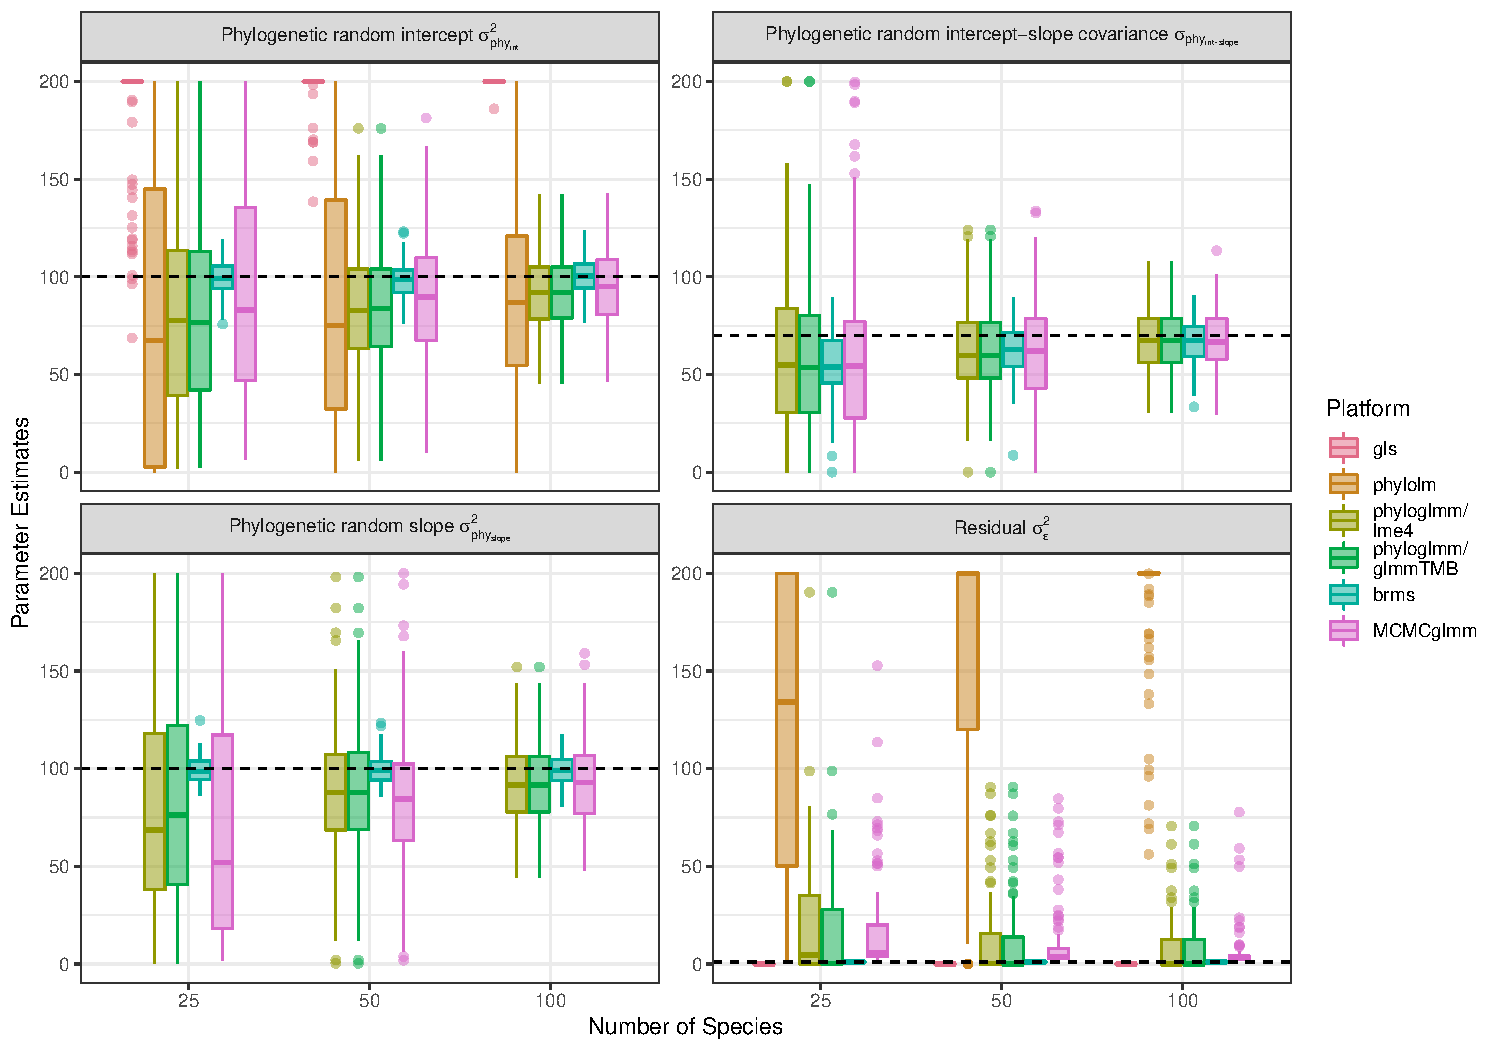
\includegraphics[scale=0.7]{./figure/ssplot.pdf}
  \caption{Comparison of single group model parameter estimates across different R packages in Table \ref{table:platform}. Total simulations $N=100$ for each category. The horizontal line shows the true value of the parameters in the simulation model. Models capable of fitting all parameters (\pkg{lme4},  \pkg{glmmTMB}, and \pkg{brms}) fit well for all parameters.
%\bmb{consider tweaking aspect ratio (slightly wider?) Consider including n=25, n=50, n=100 in x-axis tick labels (I don't have all the output data so can't rebuild figs myself ...)
%\jd{Use dashed lines (or some other gg signifier) for the insufficient approaches}
}
\label{ssplot}
\end{figure}
\end{center}
\begin{center}
\begin{figure}[H]
  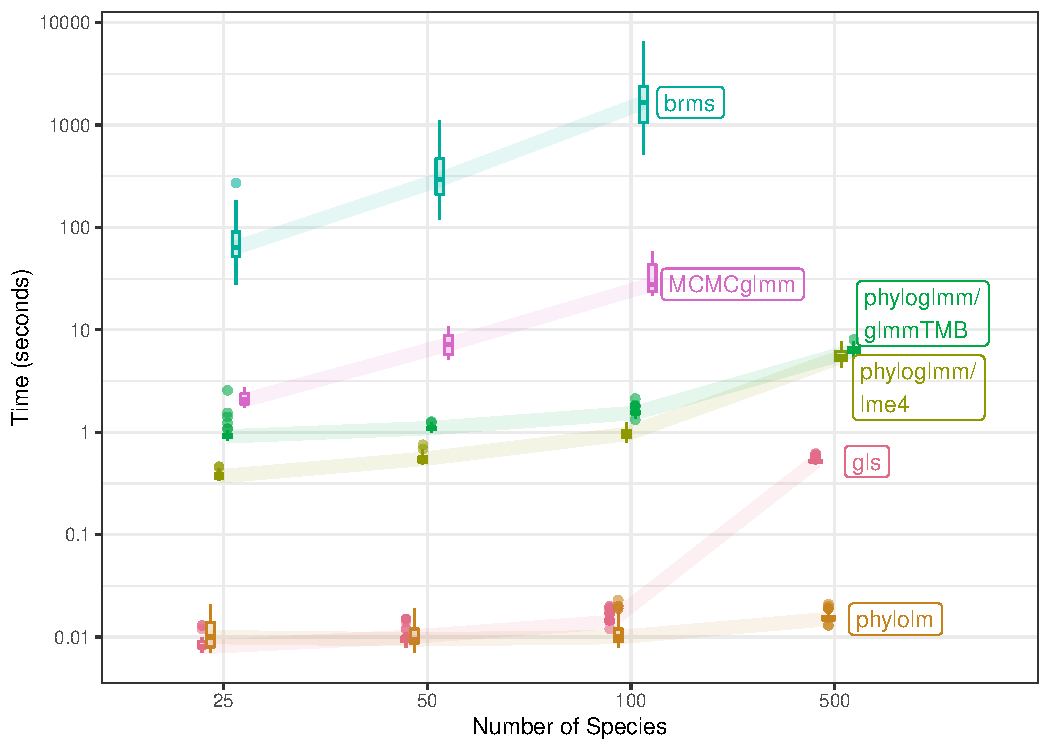
\includegraphics[scale=0.7]{./figure/sstime.pdf}
  \caption{Comparison of single-group model computational speed.}
\label{ssplot_speed}
\end{figure}
\end{center}
\begin{center}
\begin{figure}[H]
  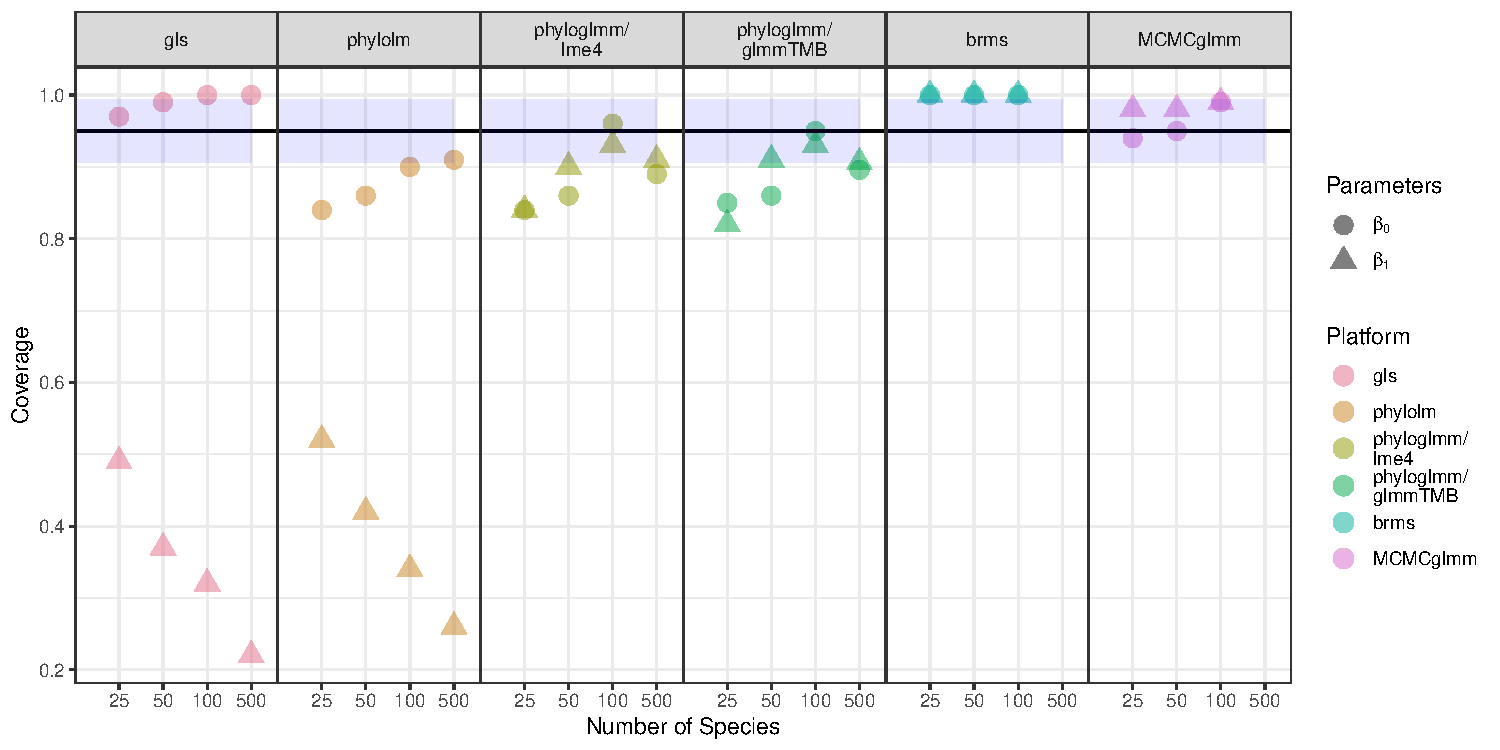
\includegraphics[scale=0.7]{./figure/sscoverage.pdf}
  \caption{Comparison of coverage probability for fixed effect parameters. Models matching the simulation model (\pkg{lme4}, \pkg{glmmTMB} and pkg{brms}) have coverage near the nominal value of 0.95. The black line shows the nominal coverage, and the blue ribbon the 95\% binomial confidence interval based on 100 simulated fits. 
%  \bmb{really picky, but maybe change grid lines or ribbon colour slightly so they're not confusable (maybe use blue ribbon with alpha=0.1?)}
  }
\label{ssplot_coverage}
\end{figure}
\end{center}

The full fitted model (which matches the simulation model that incorporates phylogenetic intercept, slope, and correlation) provides estimates with low bias (average difference between the estimated parameters and the true simulation parameters) for all parameters. 
Estimates for fixed effect parameters ($\beta_0$ and $\beta_1$) approach nominal coverage as the number of species increases for \pkg{lme4} and \pkg{glmmTMB} but not for other packages. \pkg{brms} has higher than nominal coverage (i.e., its confidence intervals are too conservative) because the prior distributions for the simulation parameters are centered at the true values (\citet{li2018fitting}).

In general, models that are insufficiently flexible to match the data (PGLM and PGLS) will lead to bias in some parameters.
PGLM (which lacks the phylogenetic slope parameter) provides reasonably good estimates for the phylogenetic intercept standard deviation parameter ($\sigma_{\mathrm{phy_{int}}}$) but overestimates the residual standard deviation; the estimates for the intercept ($\beta_0$) are slightly overconfident (coverage $\approx$ 90\% with 100 species) and the fixed slope parameter ($\beta_1$) has extremely poor coverage ($<$ 60\%).
PGLS, which uses only one parameter, combines all variation (phylogenetic intercept, slope and residual variation) into the phylogenetic intercept parameter, resulting in overestimating the phylogenetic intercept variation, over-covering for $\beta_0$, and under-covering for $\beta_1$.

\subsection*{Multi-group model simulations}

\begin{center}
\begin{figure}[H]
  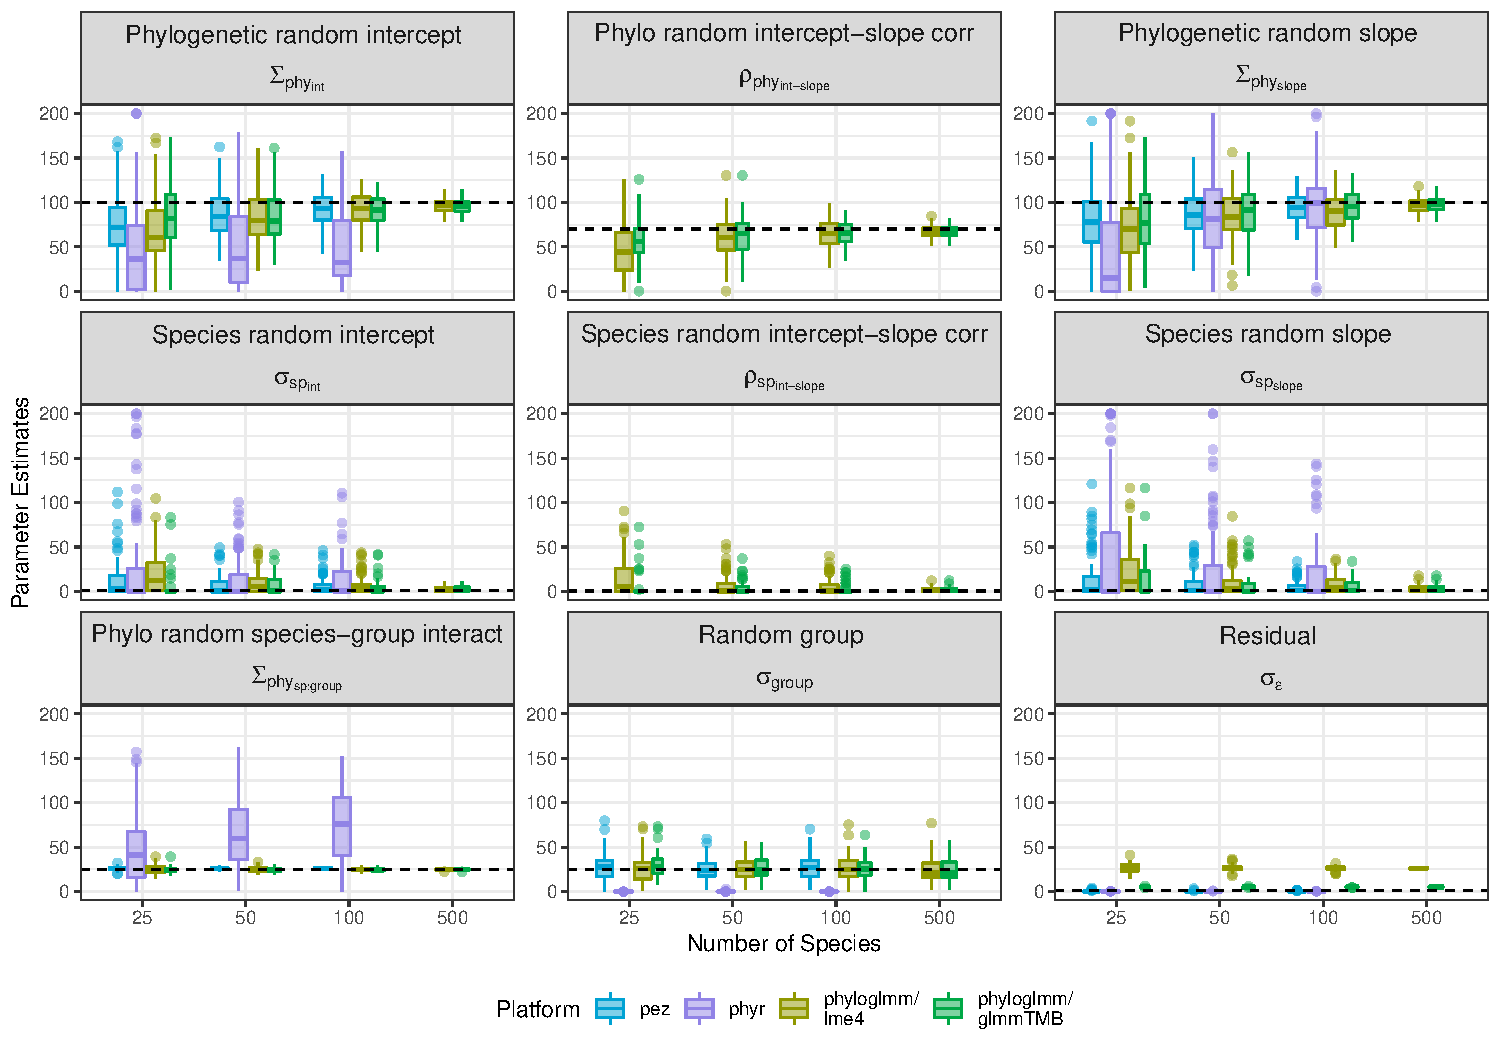
\includegraphics[scale=0.7]{./figure/msplot.pdf}
  \caption{Comparison of multi-group model parameter estimates. The horizontal line shows the true value of the parameters in the simulation model. Models capable of fitting all parameters (\pkg{lme4} and \pkg{glmmTMB}) fit well for all parameters. \pkg{pez} and \pkg{phyr} estimates for n = 100 and 500 are missing because the models did not converge within 30 minutes.
  }
  \label{msplot}
\end{figure}
\end{center}
\begin{center}
\begin{figure}[H]
  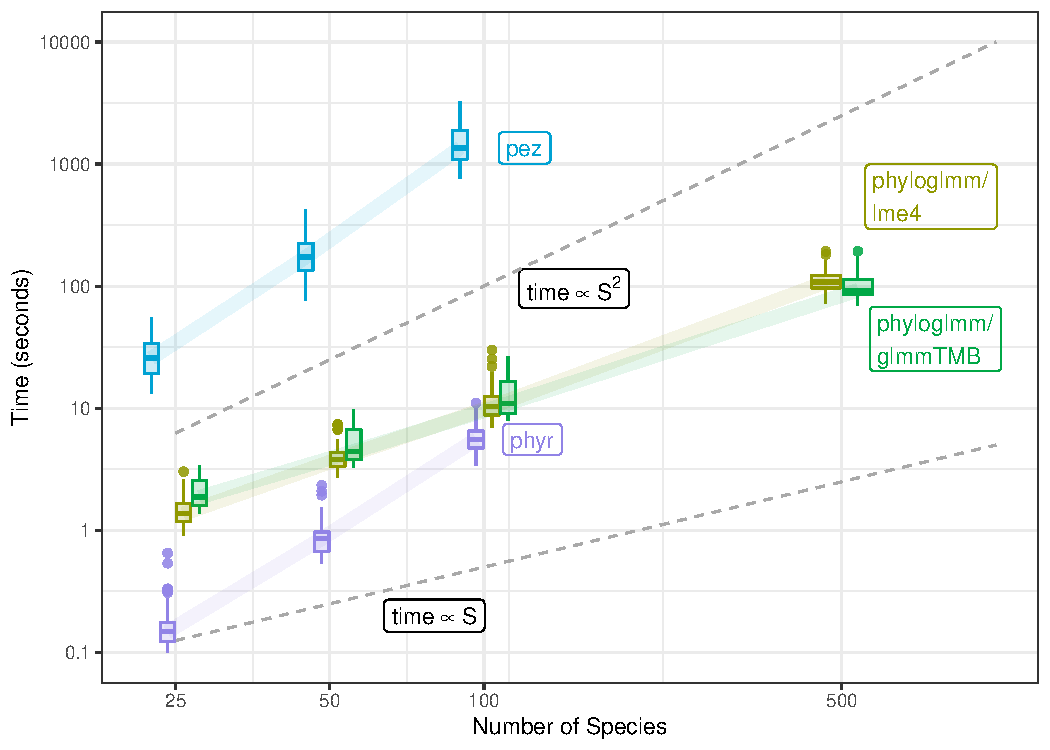
\includegraphics[scale=0.7]{./figure/mstime.pdf}
  \caption{Comparison of multi-group model computational speed.}
  \label{msplot_time}
\end{figure}
\end{center}
\begin{center}
\begin{figure}[H]
  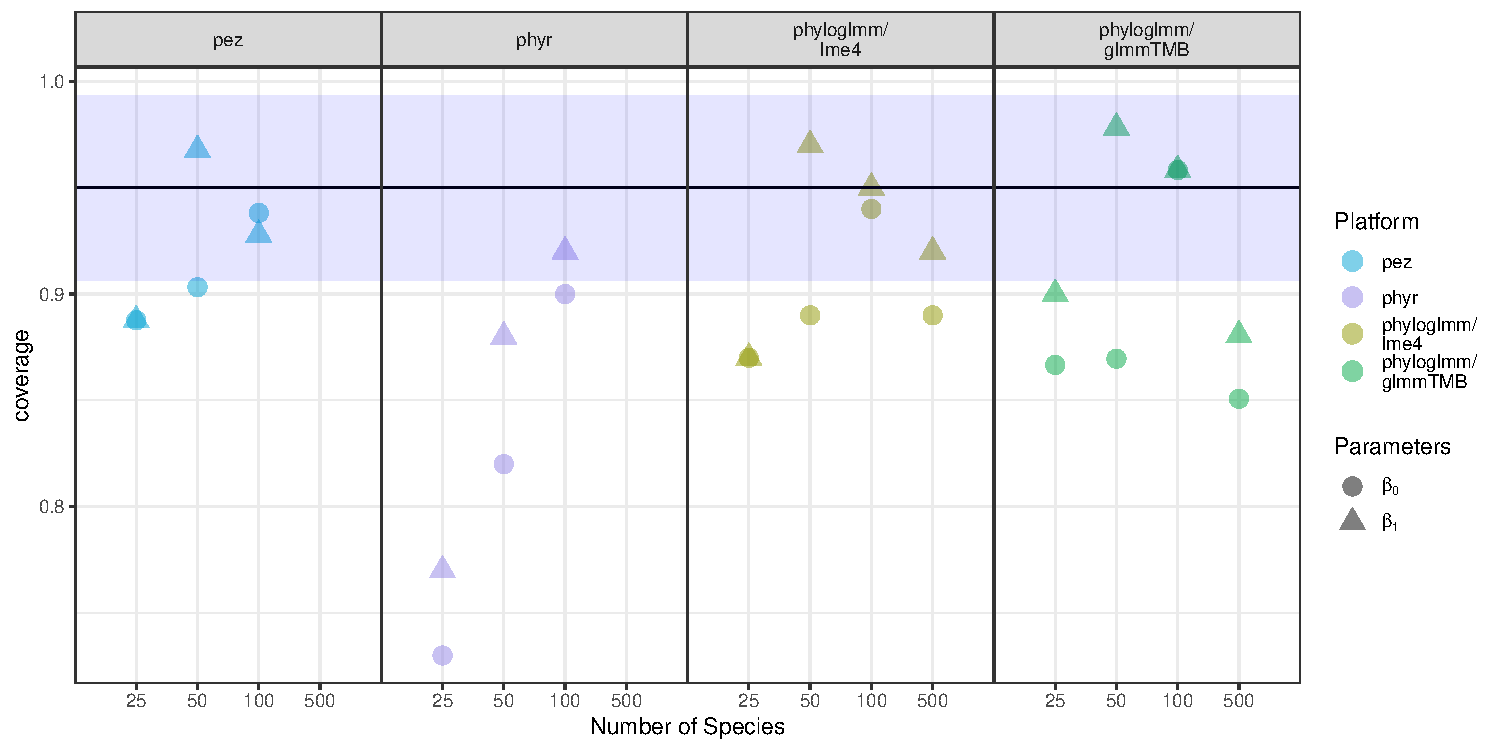
\includegraphics[scale=0.7]{./figure/mscoverage.pdf}
  \caption{Comparison of multi-group model coverage. The black line shows the nominal coverage, and the blue ribbon the 95\% binomial confidence interval based on 100 simulated fits.}
  \label{msplot_coverage}
\end{figure}
\end{center}

The multi-group model estimates are much more similar across platforms (only a subset of platforms can fit these models at all, and the fitting models are closer to the true model).
As with the single-group fits, \pkg{lme4} and \pkg{glmmTMB} match the simulation model well and provide good estimates for all parameters, except the correlation ($\sigma_{\mathrm{sp_{int-slope}}}$) for small numbers of species (i.e. n = 25 and 50).
The absence of correlations in \pkg{pez} and \pkg{phyr}'s statistical models has little effect on the other parameter estimates but leads to underestimates of the residual standard deviation (Figure \ref{msplot}).

Although the parameter estimates are similar across platforms, computational efficiency varies enormously across platforms and sample size.
Comparing our two implementations, \pkg{glmmTMB} is almost an order of magnitude faster than \pkg{lme4}.
\pkg{glmmTMB} is also faster than \pkg{pez} and \pkg{phyr}: the median time for \pkg{glmmTMB} to fit a 50-species model is $\approx$ 9, versus $\approx$ 200 seconds for \pkg{pez} and \pkg{phyr}.
\pkg{glmmTMB} takes $\approx$ 125 seconds to fit a 500-species model; it was impractical to fit 500-species models with \pkg{pez} and \pkg{phyr}.

% \bmb{Can you put a lower bound on \pkg{pez}'s computation time? How long did you take to give up? How does it scale? can you either figure out from first principles
%   or (easier) do a brute-force series of increasing sample size and
%   compute a log-log regression of time vs sample size to find the
%   approximate power?}

\section*{Discussion}

We have simulated relatively complex models containing phylogenetic variation in species intercepts and slopes, as well as within-species variation.
Comparing our fits with simple platforms for phylogenetic regression that cannot handle these complexities may seem unfair; nevertheless, our models are certainly less complex than evolutionary processes occurring in nature.
Models that cannot match the full simulations perform poorly even for the parameters they do estimate.

Even the relatively simple multi-group model described in (\ref{eq:multiple_glmm}) can incorporate many layers of complexity.
In theory, as long as we have enough data and enough computational power, models that can incorporate more of the complexity will always describe a biological system better.
However, real applications are always data-constrained.
Establishing the practical level of model complexity for a given problem and data set is an open and difficult general problem throughout statistical modeling, not just in phylogenetic studies.
%For example, should one use simple models that may be overly conservative or
% risk overfitting by using more ambitious models?
%What are the relative costs and benefits of using a step-down procedure
%starting from the most complex possible model \citep{barr2013random},
%choosing simpler models \emph{a priori} \citep{baayen2008mixed},
%or using Bayesian approaches with regularizing priors \citep{hadfield2010mcmc}?
%For predictive models, how can one appropriately evaluate out-of-sample accuracy for
%structured data \citep{roberts_cross-validation_2016}?

\subsection*{Incorporating multiple levels of variation}

Random-slopes models require appropriate observational or experimental designs (i.e., multiple measurements of traits and responses within each group) and generally require more data overall, but they are relevant over a wide range of scenarios \citep{schielzeth2008conclusions, cleasby2015quantifying,ord2010adaptation}.
Neglecting random slopes can lead to biased fixed effect estimates with inadequate coverage and inflated type~I errors \citep{schielzeth2008conclusions}.

Nevertheless, it is impossible to account for all possible complexities.
The best model --- whether using phylogenetic random effects, simple grouping, or both --- depends on the experimental design and whether there are enough data to separate different levels of variation, which can be strongly confounded.
If multiple observations are available per species, then simple methods like Pagel's $\lambda$ will confound tip variation with residual variation \citep{boettiger2013is}.
Multiple observations can be collapsed to a single value (such as the mean) per species, with analyses weighting each species by its number of observations.
Alternatively, if the within-species variance is of interest, a phylogenetic mixed model can separate tip variation from within-species variation and measurement error.
More generally, phylogenetic mixed models can be simplified to ordinary mixed models, at the cost of taxonomic detail, by simplifying the phylogenetic tree to a strictly hierarchical set of nested higher-level taxa \citep{bunnefeld2012island}). 
Users should be aware of two essential questions when fitting random-slope models: do they have enough information to practically estimate the random slopes, and what are the potential costs of ignoring them \citep{schielzeth2008conclusions}? 
% However, in the PGLMM context, as long as there's variation in the predictor among tips, there will be variation among taxa at some level, so random-slopes models will (almost always) be \emph{theoretically} identifiable.

\subsection*{Extensions and alternatives}

The range of PCMs presented here can incorporate many levels and types of phylogenetic variation.
Of course, there are further biological complexities we have neglected, such as multivariate responses; non-Brownian evolutionary processes such as the Ornstein-Uhlenbeck model \citep{butler2004phylogenetic}); and variable-rate models, which allow evolutionary rates to vary across the phylogeny.
While it cannot easily incorporate these complexities, the approach here does offer an efficient way to analyze a wide range of evolutionary scenarios.
The general principle of encoding phylogenetic structure in the random effects model matrix can be implemented with any platform that supports continuous latent variables.
Our implementation allows users to explore new ideas by fitting phylogenetic mixed models with complex random effects to large data sets.

\section*{Achnowledgements}

We would like to thank Jonathan Dushoff for thoughtful comments.
This study was funded by NSERC Discovery Grant.

\section*{Authors’ contributions}

ML and BMB conceived the ideas and designed methodology; ML and BMB implemented the code in \pkg{lme4} and \pkg{glmmTMB}; ML ran all simulations; ML and BMB analyzed the results; ML wrote the first draft. Both authors contributed critically to the drafts and gave final approval for publication.

\section*{Data Availability}

All codes are available at DOI:10.5281/zenodo.2639887.

\bibliography{phyloglmm}

\end{document}

